% IEEE figure snippets.
% Put the PDF figures in the same relative path or update the paths below.

\begin{figure*}[t]
  \centering
  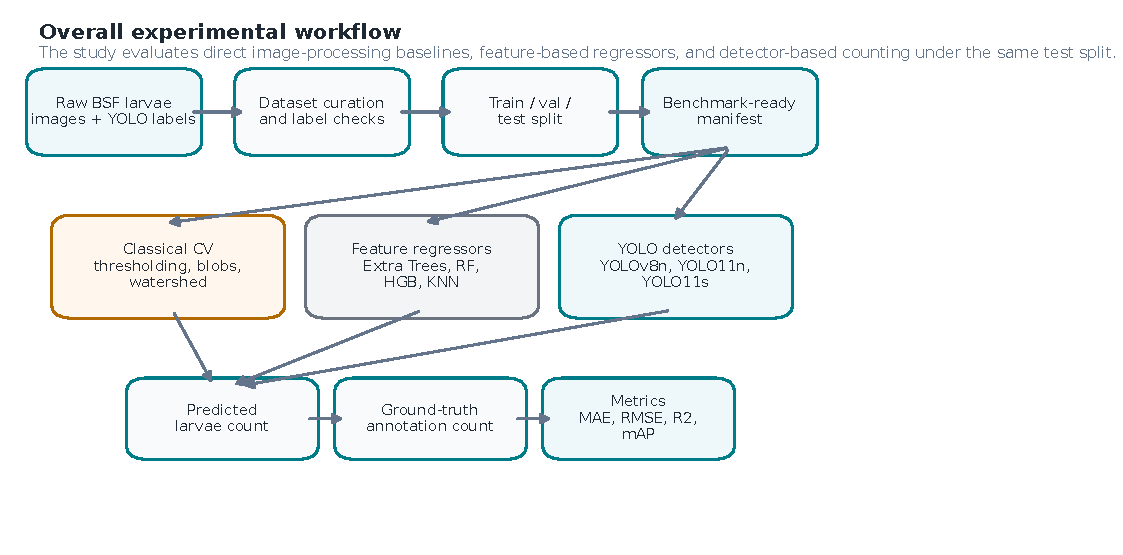
\includegraphics[width=\textwidth]{reports/paper_q4_prep/ieee_figures/fig01_methodology_flowchart.pdf}
  \caption{Overall experimental workflow. Raw BSF larvae images and YOLO-format annotations were curated into a benchmark-ready manifest, split into train, validation, and test partitions, and evaluated using classical image-processing baselines, feature-based count regressors, and YOLO detector-based counting.}
  \label{fig:methodology_workflow}
\end{figure*}

\begin{figure}[t]
  \centering
  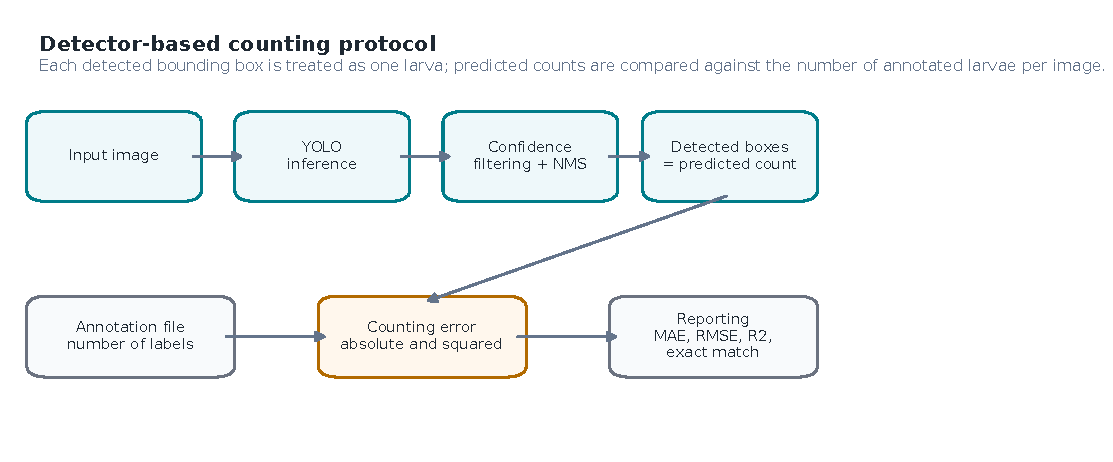
\includegraphics[width=\columnwidth]{reports/paper_q4_prep/ieee_figures/fig02_detector_counting_pipeline.pdf}
  \caption{Detector-based counting protocol. Each predicted bounding box is interpreted as one larva, and the resulting predicted count is compared with the number of annotated larvae per image.}
  \label{fig:detector_counting_protocol}
\end{figure}

\begin{figure*}[t]
  \centering
  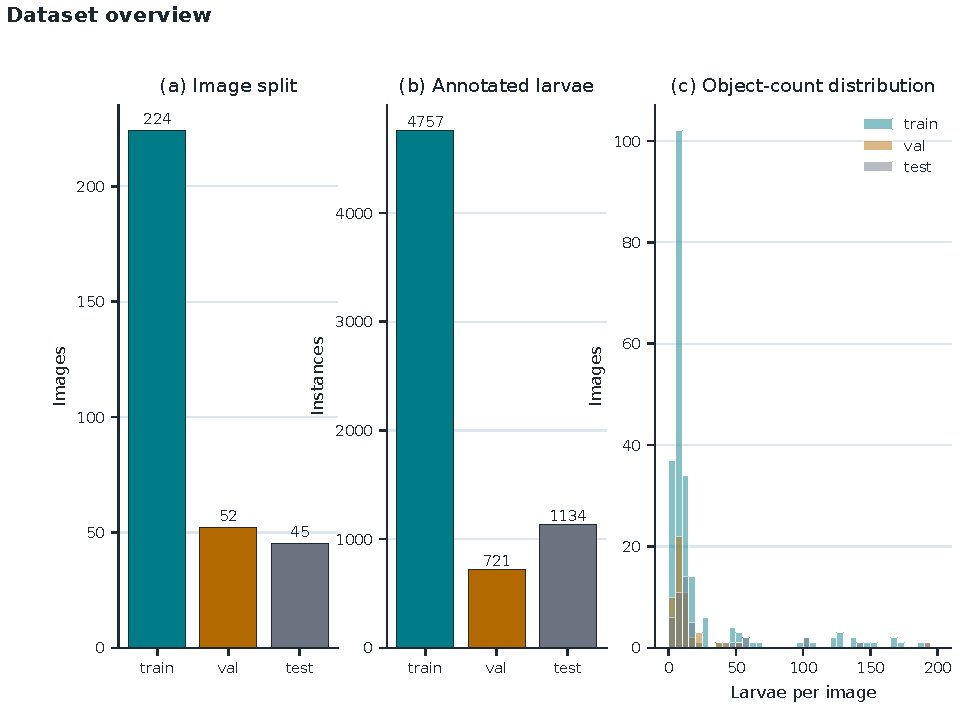
\includegraphics[width=\textwidth]{reports/paper_q4_prep/ieee_figures/fig03_dataset_overview.pdf}
  \caption{Dataset overview showing train, validation, and test image counts, annotated larvae counts, and object-count distribution.}
  \label{fig:dataset_overview}
\end{figure*}

\begin{figure}[t]
  \centering
  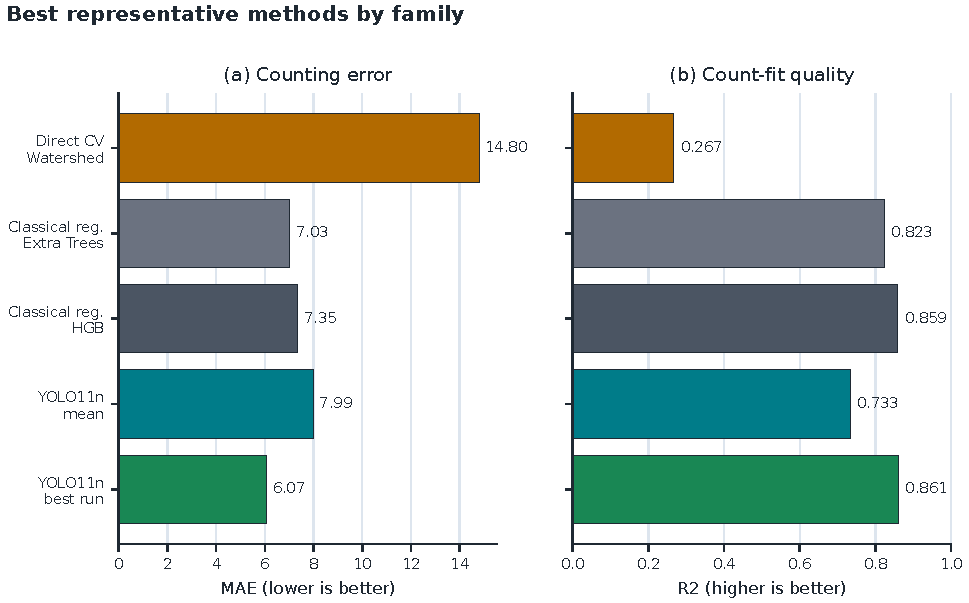
\includegraphics[width=\columnwidth]{reports/paper_q4_prep/ieee_figures/fig04_method_family_comparison.pdf}
  \caption{Best representative methods by family. Direct classical computer vision was weaker than feature-based count regressors and detector-based counting, while the best YOLO11n run achieved the lowest test MAE.}
  \label{fig:method_family_comparison}
\end{figure}

\begin{figure*}[t]
  \centering
  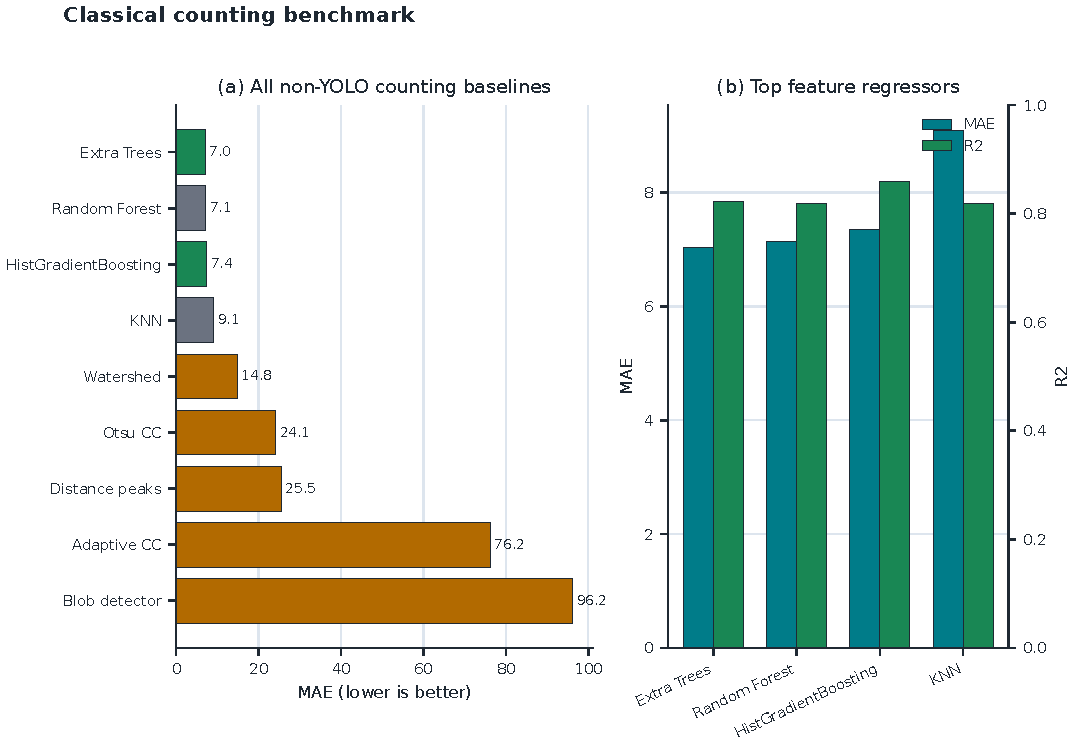
\includegraphics[width=\textwidth]{reports/paper_q4_prep/ieee_figures/fig05_classical_counting_benchmark.pdf}
  \caption{Classical counting benchmark. Feature-based regressors were the strongest non-deep-learning methods; Extra Trees produced the lowest classical MAE, while HistGradientBoosting produced the strongest classical RMSE/R2 behavior.}
  \label{fig:classical_counting_benchmark}
\end{figure*}

\begin{figure*}[t]
  \centering
  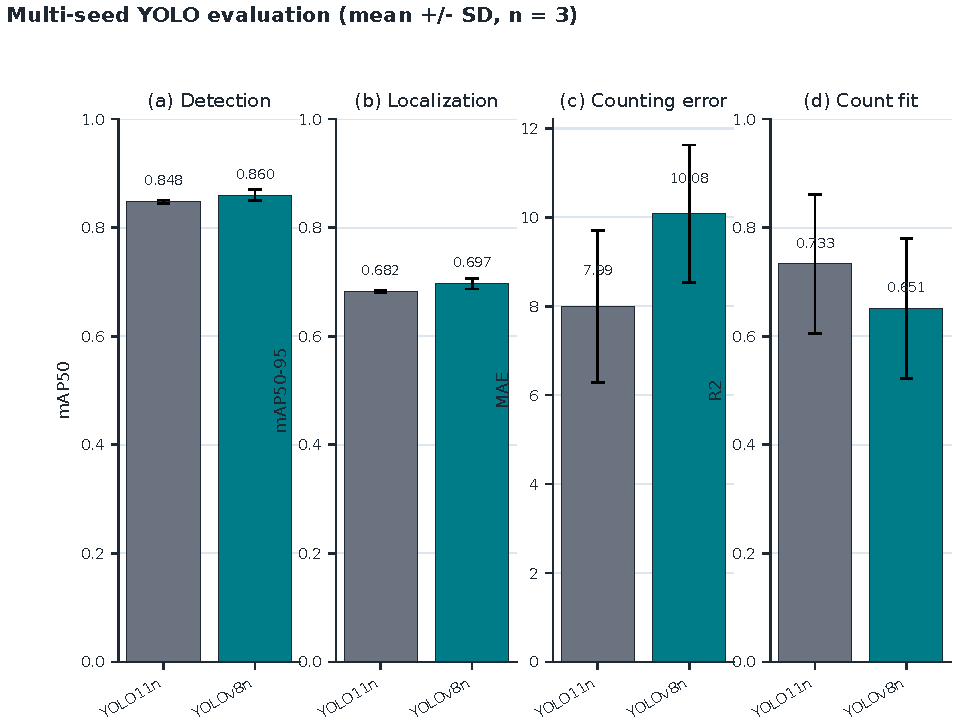
\includegraphics[width=\textwidth]{reports/paper_q4_prep/ieee_figures/fig06_yolo_multiseed_metrics.pdf}
  \caption{Multi-seed YOLO evaluation. Bars show mean and standard deviation across three random seeds for YOLOv8n and YOLO11n.}
  \label{fig:yolo_multiseed_metrics}
\end{figure*}

\begin{figure}[t]
  \centering
  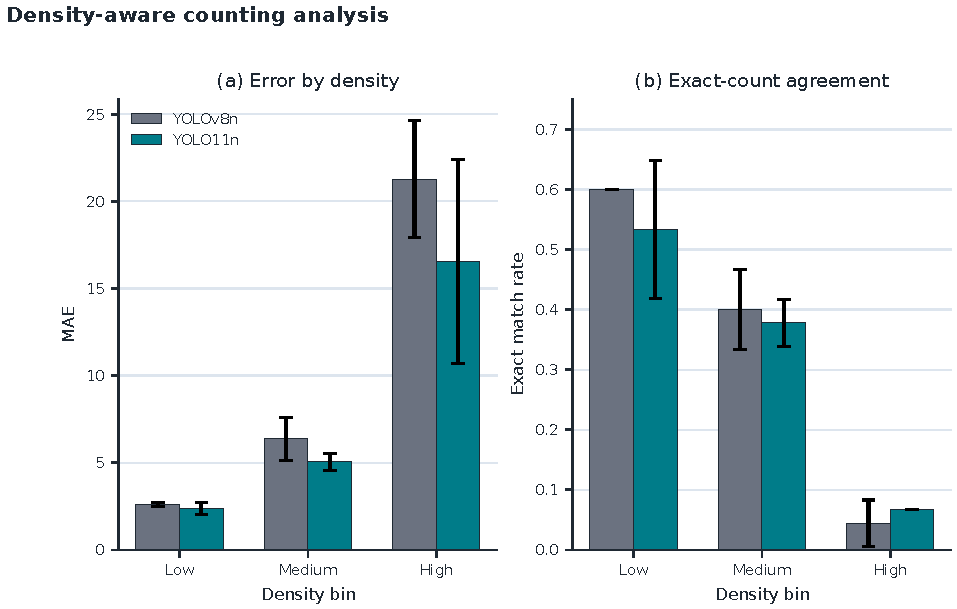
\includegraphics[width=\columnwidth]{reports/paper_q4_prep/ieee_figures/fig07_density_error_analysis.pdf}
  \caption{Density-aware counting analysis. Counting error increased substantially in high-density scenes, indicating that crowded larvae regions are the main remaining failure mode.}
  \label{fig:density_error_analysis}
\end{figure}

\begin{figure}[t]
  \centering
  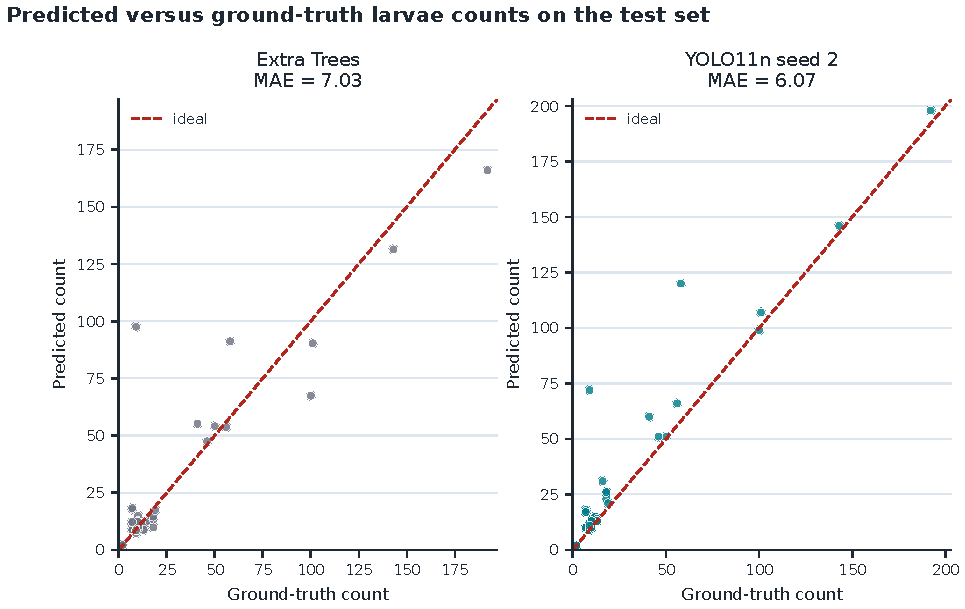
\includegraphics[width=\columnwidth]{reports/paper_q4_prep/ieee_figures/fig08_prediction_scatter.pdf}
  \caption{Predicted versus ground-truth counts for the strongest classical MAE baseline and the best detector-based single run on the test set.}
  \label{fig:prediction_scatter}
\end{figure}

\begin{figure}[t]
  \centering
  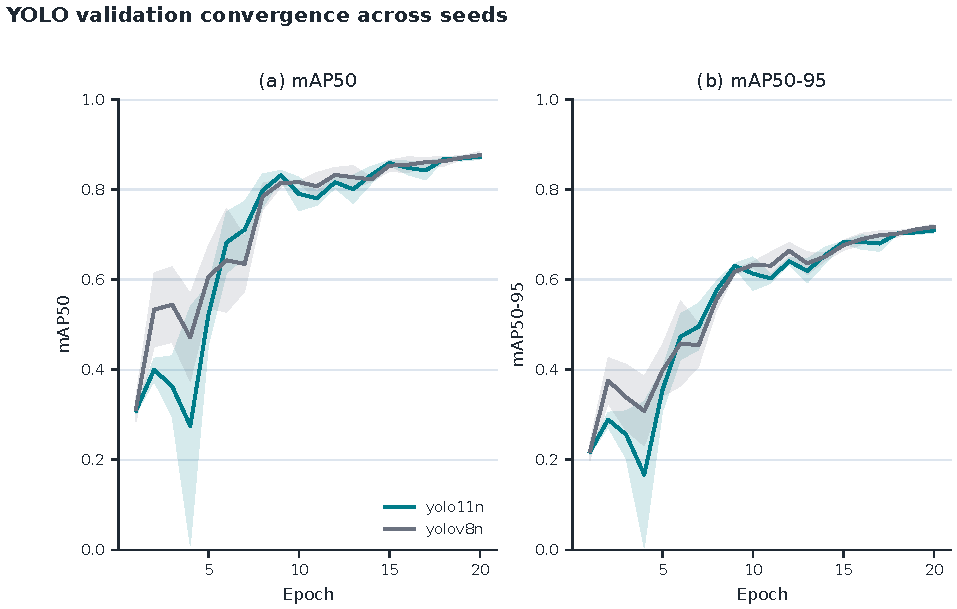
\includegraphics[width=\columnwidth]{reports/paper_q4_prep/ieee_figures/fig09_training_curves.pdf}
  \caption{YOLO validation convergence across seeds. Shaded regions represent one standard deviation across seeds.}
  \label{fig:training_curves}
\end{figure}

\begin{figure*}[t]
  \centering
  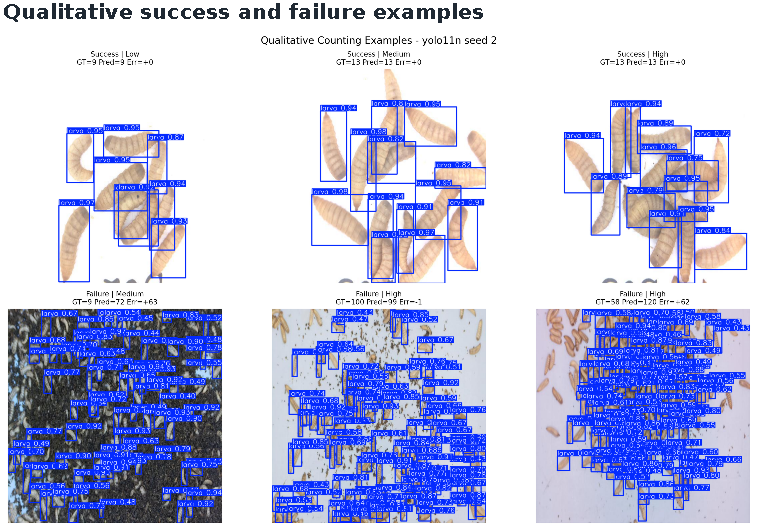
\includegraphics[width=\textwidth]{reports/paper_q4_prep/ieee_figures/fig10_qualitative_success_failure_montage.pdf}
  \caption{Qualitative success and failure examples from the best detector-based run, including exact-count successes and crowded-scene over-counting failures.}
  \label{fig:qualitative_examples}
\end{figure*}
